%==============================================================
%  EE201 -- Circuit Theory I
%  Lecture 8 : Planar Graphs, the Mesh Matrix and Mesh Currents
%  M. Mert Ankaralı, METU EEE
%
%  Compile:  ./build.sh      (or: pdflatex EE201_Lecture_8.tex, twice)
%==============================================================
\documentclass[11pt,a4paper]{article}

%-------------------- packages --------------------------------
\usepackage[T1]{fontenc}
\usepackage[utf8]{inputenc}
\usepackage[english]{babel}
\usepackage{lmodern}
\usepackage[margin=2.3cm,top=2.0cm,bottom=1.9cm,headheight=14pt,headsep=9pt]{geometry}
\usepackage{amsmath,amssymb}
\usepackage{array,booktabs,tabularx}
\usepackage{enumitem}
\usepackage[table]{xcolor}
\usepackage{fancyhdr}
\usepackage{titlesec}
\usepackage{graphicx}
\usepackage[most]{tcolorbox}
\usepackage{tikz}
\usepackage[american,siunitx]{circuitikz}
\usetikzlibrary{matrix,arrows.meta,positioning,calc,decorations.pathmorphing,decorations.pathreplacing,decorations.markings,patterns,shapes.geometric}
\usepackage[colorlinks=true,allcolors=metured,breaklinks=true]{hyperref}

%-------------------- colour system ---------------------------
% One colour per physical quantity, used identically in the slides.
\definecolor{metured}{RGB}{155,27,48}    % headings, structure
\definecolor{metugray}{RGB}{88,89,91}
\definecolor{ccur}{RGB}{0,102,170}       % CURRENT  -- blue
\definecolor{cvolt}{RGB}{214,120,0}      % VOLTAGE  -- orange
\definecolor{cpow}{RGB}{23,128,74}       % POWER / ENERGY -- green
\definecolor{ccharge}{RGB}{124,60,160}   % CHARGE   -- purple
\definecolor{cflux}{RGB}{0,138,138}      % FLUX -- teal
\definecolor{boxgray}{RGB}{245,245,245}
\definecolor{copper}{RGB}{184,98,30}

\newcommand{\Icol}[1]{\textcolor{ccur}{#1}}
\newcommand{\Vcol}[1]{\textcolor{cvolt}{#1}}
\newcommand{\Pcol}[1]{\textcolor{cpow}{#1}}
\newcommand{\Qcol}[1]{\textcolor{ccharge}{#1}}
\newcommand{\Fcol}[1]{\textcolor{cflux}{#1}}

%-------------------- units (no siunitx dependency) -----------
\newcommand{\uni}[1]{\,\mathrm{#1}}
\newcommand{\A}{\uni{A}}   \newcommand{\V}{\uni{V}}
\newcommand{\W}{\uni{W}}   \newcommand{\J}{\uni{J}}
\newcommand{\Cb}{\uni{C}}  \newcommand{\s}{\uni{s}}
\newcommand{\Sie}{\uni{S}} \newcommand{\Wb}{\uni{Wb}}

%-------------------- layout ----------------------------------
\pagestyle{fancy}
\fancyhf{}
\lhead{\small\textcolor{metugray}{EE201 -- Circuit Theory I}}
\rhead{\small\textcolor{metugray}{Lecture 8: Planar Graphs, the Mesh Matrix and Mesh Currents}}
\cfoot{\small\thepage}
\renewcommand{\headrulewidth}{0.4pt}

\titleformat{\section}{\large\bfseries\color{metured}}{\thesection.}{0.6em}{}
\titleformat{\subsection}{\normalsize\bfseries\color{metugray}}{\thesubsection.}{0.6em}{}
\titlespacing*{\section}{0pt}{1.4ex plus .3ex}{0.7ex}
\titlespacing*{\subsection}{0pt}{1.1ex plus .2ex}{0.5ex}

\setlist[itemize]{itemsep=2pt,topsep=3pt,parsep=0pt,leftmargin=1.5em}
\setlist[enumerate]{itemsep=2pt,topsep=3pt,parsep=0pt,leftmargin=1.7em}
\setlength{\parindent}{0pt}
\setlength{\parskip}{0.7ex plus .1ex}
\raggedbottom
\widowpenalty=10000
\clubpenalty=10000
\brokenpenalty=10000

%-------------------- boxes -----------------------------------
\newtcolorbox{definitionbox}[1]{enhanced,
  colback=metured!4, colframe=metured, boxrule=0.9pt,
  fonttitle=\bfseries, title={#1}, arc=2pt,
  left=7pt,right=7pt,top=5pt,bottom=5pt, before skip=7pt, after skip=7pt,
  before upper={\setlength{\parskip}{0.6ex plus .1ex}}}

\newtcolorbox{ideabox}[1][Key idea]{enhanced,
  colback=ccur!5, colframe=ccur, boxrule=0.9pt,
  fonttitle=\bfseries, title={#1}, arc=2pt,
  left=7pt,right=7pt,top=5pt,bottom=5pt, before skip=7pt, after skip=7pt,
  before upper={\setlength{\parskip}{0.6ex plus .1ex}}}

\newtcolorbox{examplebox}[1][Example]{enhanced,
  colback=cpow!4, colframe=cpow, boxrule=0.9pt,
  fonttitle=\bfseries, title={#1}, arc=2pt,
  left=7pt,right=7pt,top=5pt,bottom=5pt, before skip=7pt, after skip=7pt,
  before upper={\setlength{\parskip}{0.6ex plus .1ex}}}

\newtcolorbox{cautionbox}[1][Careful]{enhanced,
  colback=cvolt!6, colframe=cvolt, boxrule=0.9pt,
  fonttitle=\bfseries, title={#1}, arc=2pt,
  left=7pt,right=7pt,top=5pt,bottom=5pt, before skip=7pt, after skip=7pt,
  before upper={\setlength{\parskip}{0.6ex plus .1ex}}}

%-------------------- circuitikz defaults ---------------------
\ctikzset{bipoles/length=0.9cm, color=black,
          label/align=straight,
          bipoles/generic/height=0.28, bipoles/generic/width=0.62}
\tikzset{
  iar/.style={-{Stealth[length=2.2mm]}, ccur, thick},
  pol/.style={font=\small, text=cvolt},
  glab/.style={font=\footnotesize, text=metured},
  ttl/.style={font=\scriptsize\bfseries, text=metugray},
  capn/.style={font=\scriptsize, text=metugray, align=center},
  bigarr/.style={-{Stealth[length=3mm]}, very thick, metugray},
  gnode/.style={circle, fill=metured, inner sep=0pt, minimum size=4.4pt},
  nlab/.style={circle, draw=metured, text=metured, font=\scriptsize, inner sep=0.7pt},
  blab/.style={font=\footnotesize, text=black!80},
  gbr/.style={black!75, thick, postaction={decorate, decoration={markings,
      mark=at position 0.56 with {\arrow{Stealth[length=2.5mm]}}}}},
  hal/.style={draw=cpow!60, line width=6pt, opacity=0.35, line cap=round, line join=round},
  elem/.style={draw=metugray, thick, fill=metulight},
}
\definecolor{metulight}{RGB}{243,240,241}
\newcommand{\ohm}{\,\Omega}

%  A circled node number, for the text and the matrices
\newcommand{\nd}[1]{\tikz[baseline=(c.base)]\node[nlab](c){#1};}
%  Branch current arrow beside the element from #1 to #2, on side #3 (90 = left, -90 = right),
%  with branch number #4
\newcommand{\brarr}[4]{%
  \draw[iar] ($(#1)!0.34!(#2)!0.34cm!#3:(#2)$) -- ($(#1)!0.66!(#2)!0.34cm!#3:(#2)$);
  \node[blab] at ($(#1)!0.5!(#2)!0.66cm!#3:(#2)$) {#4};}
%  A straight graph branch from #1 to #2, number #4 on side #3
\newcommand{\gbranch}[4]{%
  \draw[gbr] (#1) -- (#2);
  \node[blab] at ($(#1)!0.5!(#2)!0.28cm!#3:(#2)$) {#4};}
%  An incidence matrix with node labels on the left and branch numbers on top.
%  #1 name, #2 number of columns, #3 node labels, #4 rows (entries separated by \&)
\newcommand{\incmat}[4]{%
  \begin{tikzpicture}[baseline={([yshift=-0.6ex]#1.center)}]
    \matrix (#1) [matrix of math nodes, ampersand replacement=\&,
                  left delimiter={[}, right delimiter={]}, inner sep=1pt,
                  column sep=0.45em,
                  nodes={text width=1.35em, align=right, minimum height=1.25em,
                         inner sep=1pt}] {#4};
    \foreach \j in {1,...,#2}
      \node[font=\scriptsize, text=metugray, anchor=south east, inner sep=1pt]
        at ([yshift=2pt]#1-1-\j.north east) {\j};
    \foreach \lab [count=\i] in {#3}
      \node[nlab, left=11pt] at (#1.west |- #1-\i-1) {\lab};
  \end{tikzpicture}}
%  Same, with explicit column labels: #1 name, #2 column labels, #3 row labels,
%  #4 rows, #5 extra TikZ code
\newcommand{\incmatc}[5]{%
  \begin{tikzpicture}[baseline={([yshift=-0.6ex]#1.center)}]
    \matrix (#1) [matrix of math nodes, ampersand replacement=\&,
                  left delimiter={[}, right delimiter={]}, inner sep=1pt,
                  column sep=0.45em,
                  nodes={text width=1.35em, align=right, minimum height=1.25em,
                         inner sep=1pt}] {#4};
    \foreach \lab [count=\j] in {#2}
      \node[font=\scriptsize, text=metugray, anchor=south east, inner sep=1pt]
        at ([yshift=2pt]#1-1-\j.north east) {\lab};
    \foreach \lab [count=\i] in {#3}
      \node[nlab, left=11pt] at (#1.west |- #1-\i-1) {\lab};
    #5
  \end{tikzpicture}}
%  A two-winding ideal-transformer symbol between (#1,0)--(#1,#2) on the left and
%  (#1+1.6,0)--(#1+1.6,#2) on the right; dots at the top of both windings.
\newcommand{\xfmr}[2]{%
  \begin{scope}[xshift=#1 cm]
    \ctikzset{bipoles/length=1.35cm}
    \draw (0,0) to[L] (0,#2);
    \draw (1.6,#2) to[L] (1.6,0);
    \draw[line width=1.1pt, metugray] (0.72,-0.05) -- (0.72,#2+0.05);
    \draw[line width=1.1pt, metugray] (0.88,-0.05) -- (0.88,#2+0.05);
    \fill (0.36,#2-0.2) circle (2.1pt);
    \fill (1.24,#2-0.2) circle (2.1pt);
  \end{scope}}
%  The four node positions of the bridge circuit N
\newcommand{\bridgecoords}{%
  \coordinate (n1) at (0,1.7);  \coordinate (n2) at (-1.5,0);
  \coordinate (n3) at (1.5,0);  \coordinate (n4) at (0,-1.7);}
\newcommand{\bridgenodes}{%
  \foreach \k/\pos in {1/above, 2/left, 3/right, 4/below}
    {\fill[metured] (n\k) circle (2.2pt); \node[nlab, \pos=3pt] at (n\k) {\k};}}

\newcommand{\bridgegraph}{%
  \gbranch{n1}{n2}{-90}{1}  \gbranch{n1}{n3}{90}{2}  \gbranch{n3}{n2}{-90}{3}
  \gbranch{n2}{n4}{-90}{4}  \gbranch{n3}{n4}{90}{5}
  \draw[gbr] (n4) to[out=180, in=180, looseness=2.3] (n1);
  \node[blab] at (-2.55,0) {6};
  \bridgenodes}

%  A graph branch from #1 to #2 with its branch voltage: + near the tail, - near the head,
%  v_#4 in the middle; #3 = auto=left or auto=right picks the side
\newcommand{\gvbranch}[4]{%
  \draw[gbr] (#1) --
    node[pos=0.27, #3, pol, inner sep=1pt] {$+$}
    node[pos=0.5, #3, font=\small, text=cvolt, inner sep=2.5pt] {$v_{#4}$}
    node[pos=0.73, #3, pol, inner sep=1pt] {$-$} (#2);}
\newcommand{\bridgevgraph}{%
  \gvbranch{n1}{n2}{auto=right}{1}  \gvbranch{n1}{n3}{auto=left}{2}
  \gvbranch{n3}{n2}{auto=right}{3}  \gvbranch{n2}{n4}{auto=right}{4}
  \gvbranch{n3}{n4}{auto=left}{5}
  \draw[gbr] (n4) to[out=180, in=180, looseness=2.3]
    node[pos=0.22, left, pol, inner sep=2pt] {$+$}
    node[pos=0.5, left, font=\small, text=cvolt] {$v_6$}
    node[pos=0.78, left, pol, inner sep=2pt] {$-$} (n1);
  \bridgenodes}
%  One branch, for the definition: + at the tail, - at the head, current along the arrow
\newcommand{\onebranch}{%
  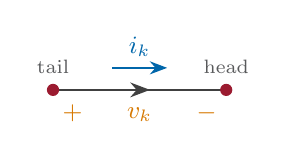
\begin{tikzpicture}[baseline=-0.6ex]
    \coordinate (p) at (0,0); \coordinate (q) at (2.2,0);
    \draw[gbr] (p) -- (q);
    \fill[metured] (p) circle (2.2pt); \fill[metured] (q) circle (2.2pt);
    \node[pol] at (0.25,-0.3) {$+$}; \node[pol] at (1.95,-0.3) {$-$};
    \node[font=\small, text=cvolt] at (1.1,-0.32) {$v_k$};
    \draw[iar] (0.75,0.28) -- (1.45,0.28); \node[font=\small, text=ccur] at (1.1,0.55) {$i_k$};
    \node[font=\scriptsize, text=metugray] at (0,0.3) {tail};
    \node[font=\scriptsize, text=metugray] at (2.2,0.3) {head};
  \end{tikzpicture}}

%==============================================================
%-------------------- Lecture 8 additions ---------------------
\tikzset{mlabst/.style={draw=ccur, text=ccur, fill=white, rounded corners=1.5pt,
                        inner sep=1.2pt, font=\scriptsize\bfseries}}
%  A boxed mesh number, for the text
\newcommand{\mlab}[1]{\tikz[baseline=(c.base)]\node[mlabst](c){#1};}
%  A clockwise mesh arrow at (#2,#3) with mesh number #4; optional radius #1
\newcommand{\meshcw}[4][0.32]{%
  \draw[ccur, thick, -{Stealth[length=2mm]}] ($(#2,#3)+(150:#1)$)
    arc[start angle=150, end angle=-150, radius=#1];
  \node[mlabst] at (#2,#3) {#4};}
%  The three inner meshes of the bridge graph (after \bridgecoords)
\newcommand{\bridgemeshes}{%
  \meshcw[0.3]{0}{0.82}{1} \meshcw[0.3]{0}{-0.78}{2} \meshcw[0.24]{-1.55}{0.66}{3}}
\newcommand{\fillmeshA}[1][]{\fill[ccur!14, #1] (n1) -- (n2) -- (n3) -- cycle;}
\newcommand{\fillmeshB}[1][]{\fill[ccur!14, #1] (n2) -- (n3) -- (n4) -- cycle;}
\newcommand{\fillmeshC}[1][]{\fill[ccur!14, #1] (n4) to[out=180, in=180, looseness=2.3] (n1) -- (n2) -- cycle;}
%  The bridge graph drawn as a square: both diagonals cross
%  Separable / nonseparable pictures: before and after removing one node.
%  Removed node: open grey circle; removed branches: dashed grey.
\tikzset{gone/.style={gray!55, thick, dash pattern=on 2.5pt off 2pt},
  gonenode/.style={gray!70, thick, fill=white},
  gonelab/.style={nlab, draw=gray!70, text=gray!70}}
\newcommand{\twotricoords}{%
  \coordinate (c) at (1.6,0.8);
  \coordinate (a1) at (0,1.6); \coordinate (a2) at (0,0);
  \coordinate (b1) at (3.2,1.6); \coordinate (b2) at (3.2,0);}
\newcommand{\twotri}{%
  \twotricoords
  \draw[black!75, thick] (c) -- (a1) -- (a2) -- cycle;
  \draw[black!75, thick] (c) -- (b1) -- (b2) -- cycle;
  \foreach \p in {a1,a2,b1,b2,c} \fill[metured] (\p) circle (2.2pt);}
\newcommand{\twotricut}{%
  \twotricoords
  \draw[gone] (a1) -- (c) -- (a2);  \draw[gone] (b1) -- (c) -- (b2);
  \draw[cvolt, very thick] (a1) -- (a2);  \draw[ccur, very thick] (b1) -- (b2);
  \foreach \p in {a1,a2,b1,b2} \fill[metured] (\p) circle (2.2pt);
  \draw[gonenode] (c) circle (2.6pt);}
%  N with node 2 removed: branches 1, 3, 4 go; 2, 5, 6 stay (one piece)
\newcommand{\bridgecut}{%
  \bridgecoords
  \draw[gone] (n1) -- (n2);  \draw[gone] (n3) -- (n2);  \draw[gone] (n2) -- (n4);
  \begin{scope}[gbr/.append style={ccur, very thick}]
    \gbranch{n1}{n3}{90}{2}  \gbranch{n3}{n4}{90}{5}
    \draw[gbr] (n4) to[out=180, in=180, looseness=2.3] (n1);
  \end{scope}
  \node[blab] at (-2.55,0) {6};
  \foreach \k/\pos in {1/above, 3/right, 4/below}
    {\fill[metured] (n\k) circle (2.2pt); \node[nlab, \pos=3pt] at (n\k) {\k};}
  \draw[gonenode] (n2) circle (2.6pt);
  \node[gonelab, left=3pt] at (n2) {2};}
%  Separable vs nonseparable, before and after removing a node. #1, #3: extra options
%  for the two "after" pictures; #2, #4: for the removed parts drawn in them
%  (overlay styles on slides, empty in the notes)
\newcommand{\nsepfigure}[4]{%
  \begin{tikzpicture}[scale=0.8]
    \begin{scope}
      \twotri
      \node[ttl] at (1.6,-1.2) {separable};
    \end{scope}
    \begin{scope}[#1]
      \draw[bigarr] (3.6,0.8) -- (4.4,0.8);
      \node[capn] at (4.0,1.35) {remove\\ centre};
      \begin{scope}[xshift=4.8cm, gone/.append style={#2}, gonenode/.append style={#2}]
        \twotricut
      \end{scope}
      \node[ttl] at (6.4,-1.2) {\textcolor{cvolt}{two} \textcolor{ccur}{pieces}};
    \end{scope}
    \draw[metugray!50] (8.7,-1.4) -- (8.7,2.3);
    \begin{scope}[xshift=11.0cm, yshift=0.8cm, scale=0.75, transform shape]
      \bridgecoords \bridgegraph
    \end{scope}
    \node[ttl] at (10.6,-1.2) {nonseparable (bridge)};
    \begin{scope}[#3]
      \draw[bigarr] (12.55,0.8) -- (13.45,0.8);
      \node[capn] at (13.0,1.35) {remove\\ node 2};
      \begin{scope}[xshift=15.9cm, yshift=0.8cm, scale=0.75, transform shape,
                    gone/.append style={#4}, gonenode/.append style={#4},
                    gonelab/.append style={#4}]
        \bridgecut
      \end{scope}
      \node[ttl] at (15.5,-1.2) {\textcolor{ccur}{still one piece}};
    \end{scope}
  \end{tikzpicture}}
\newcommand{\squarekfour}{%
  \coordinate (s1) at (0,2); \coordinate (s3) at (2,2);
  \coordinate (s4) at (2,0); \coordinate (s2) at (0,0);
  \foreach \u/\v/\k/\lp in {s1/s2/1/left, s1/s3/2/above, s2/s4/4/below, s3/s4/5/right}
    \draw[black!75, thick] (\u) -- (\v) node[midway, \lp, blab] {\k};
  \draw[black!75, thick] (s3) -- (s2) node[pos=0.25, above left, blab, inner sep=1pt] {3};
  \draw[black!75, thick] (s4) -- (s1) node[pos=0.25, above right, blab, inner sep=1pt] {6};
  \foreach \k/\pos in {1/above left, 2/below left, 3/above right, 4/below right}
    {\fill[metured] (s\k) circle (2.2pt); \node[nlab, \pos=1pt] at (s\k) {\k};}}
%  The circuit of the Tellegen example (10 V, 2, 4, 12 ohm), with current references
%  A hop (bump): the wire passes over another one without touching it.
%  \hopseg{P}{X}{Q}: from P to Q, jumping at the crossing point X
\newcommand{\hopr}{0.22cm}
\newcommand{\hopseg}[3]{%
  ($(#2)!\hopr!(#1)$) to[bend left=90, looseness=1.55] ($(#2)!\hopr!(#3)$)}
%  The square drawing of the bridge graph, branch 6 hopping over branch 3
\newcommand{\squarehop}{%
  \coordinate (s1) at (0,2); \coordinate (s3) at (2,2);
  \coordinate (s4) at (2,0); \coordinate (s2) at (0,0);
  \coordinate (sx) at (1,1);
  \foreach \u/\v/\k/\lp in {s1/s2/1/left, s1/s3/2/above, s2/s4/4/below, s3/s4/5/right}
    \draw[black!75, thick] (\u) -- (\v) node[midway, \lp, blab] {\k};
  \draw[black!75, thick] (s3) -- (s2) node[pos=0.25, above left, blab, inner sep=1pt] {3};
  \draw[copper, very thick] (s4) -- \hopseg{s4}{sx}{s1} -- (s1);
  \node[blab, text=copper] at (1.62,0.62) {6};
  \foreach \k/\pos in {1/above left, 2/below left, 3/above right, 4/below right}
    {\fill[metured] (s\k) circle (2.2pt); \node[nlab, \pos=1pt] at (s\k) {\k};}}
%  The nonplanar hexagon graph with as few hops as possible: one diagonal goes around
%  the outside, and one hop is still left
\newcommand{\hexhop}{%
  \foreach \a/\n in {0/a,60/b,120/c,180/d,240/e,300/f} \coordinate (\n) at (\a:1.15);
  \draw[black!75, thick] (a) -- (b) -- (c) -- (d) -- (e) -- (f) -- cycle;
  \draw[black!75, thick] (a) -- (d);
  \draw[black!75, thick] (b) .. controls (3.1,2.2) and (0.6,-3.3) .. (e);
  \draw[copper, very thick] (c) -- \hopseg{c}{0,0}{f} -- (f);
  \foreach \n in {a,b,c,d,e,f} \fill[metured] (\n) circle (2.2pt);}
%  The same graph in 3D: hexagon on a board, diagonals lifted to different heights.
%  #1: the x, y, z unit vectors of the view
\newcommand{\hexthreeD}[1]{%
  \begin{scope}[#1]
    \fill[metulight] (-1.55,-1.55,0) -- (1.55,-1.55,0) -- (1.55,1.55,0) -- (-1.55,1.55,0) -- cycle;
    \draw[gray!45] (-1.55,-1.55,0) -- (1.55,-1.55,0) -- (1.55,1.55,0) -- (-1.55,1.55,0) -- cycle;
    \foreach \a in {0,60,...,300}
      \draw[black!75, thick] ({1.15*cos(\a)},{1.15*sin(\a)},0) -- ({1.15*cos(\a+60)},{1.15*sin(\a+60)},0);
    \draw[black!75, thick] ({1.15*cos(120)},{1.15*sin(120)},0) -- ({-1.15*cos(120)},{-1.15*sin(120)},0);
    \foreach \a/\h in {0/0.6, 60/1.15}
      \draw[copper, very thick] plot[domain=0:1, samples=31, variable=\t]
        ({1.15*cos(\a)*(1-2*\t)},{1.15*sin(\a)*(1-2*\t)},{\h*sin(180*\t)});
    \foreach \a in {0,60,...,300} \fill[metured] ({1.15*cos(\a)},{1.15*sin(\a)},0) circle (2.2pt);
  \end{scope}}
\tikzset{
  view top/.style={x={(1cm,0cm)}, y={(0cm,1cm)}, z={(0cm,0cm)}},
  view oblique/.style={x={(0.9cm,-0.32cm)}, y={(0.9cm,0.32cm)}, z={(0cm,0.95cm)}},
  view side/.style={x={(1cm,0cm)}, y={(0.22cm,0.1cm)}, z={(0cm,0.95cm)}},
}
\newcommand{\tcircuit}[1]{%
\begin{tikzpicture}[scale=#1]
  \draw (0,0) to[american voltage source, invert] (0,2.2);
  \node[font=\small, left] at (-0.45,1.1) {$10\V$};
  \draw (0,2.2) to[R] (2.6,2.2);
  \node[font=\small] at (1.3,2.62) {$2\ohm$};
  \draw (2.6,2.2) -- (4.4,2.2);
  \draw (2.6,2.2) to[R] (2.6,0);
  \node[font=\small, right] at (2.85,1.75) {$4\ohm$};
  \draw (4.4,2.2) to[R] (4.4,0);
  \node[font=\small, right] at (4.65,1.1) {$12\ohm$};
  \draw (4.4,0) -- (0,0);
  \draw[iar] (0.55,0.7) -- (0.55,1.5);  \node[font=\small, text=ccur] at (0.85,1.1) {$i_1$};
  \draw[iar] (0.85,1.8) -- (1.75,1.8);  \node[font=\small, text=ccur] at (1.3,1.5) {$i_2$};
  \draw[iar] (2.25,1.45) -- (2.25,0.75); \node[font=\small, text=ccur] at (1.95,1.1) {$i_3$};
  \draw[iar] (4.05,1.45) -- (4.05,0.75); \node[font=\small, text=ccur] at (3.75,1.1) {$i_4$};
  \foreach \x/\y/\k/\pos in {0/2.2/1/above left, 2.6/2.2/2/above, 1.3/0/3/below}
    {\fill[metured] (\x,\y) circle (2.2pt); \node[nlab, \pos=2pt] at (\x,\y) {\k};}
  \meshcw[0.28]{1.3}{0.65}{1}
  \meshcw[0.28]{3.3}{0.6}{2}
\end{tikzpicture}}
%  A mesh matrix: like \incmat, with mesh numbers as row labels
\newcommand{\incmatm}[4]{%
  \begin{tikzpicture}[baseline={([yshift=-0.6ex]#1.center)}]
    \matrix (#1) [matrix of math nodes, ampersand replacement=\&,
                  left delimiter={[}, right delimiter={]}, inner sep=1pt,
                  column sep=0.45em,
                  nodes={text width=1.35em, align=right, minimum height=1.25em,
                         inner sep=1pt}] {#4};
    \foreach \j in {1,...,#2}
      \node[font=\scriptsize, text=metugray, anchor=south east, inner sep=1pt]
        at ([yshift=2pt]#1-1-\j.north east) {\j};
    \foreach \lab [count=\i] in {#3}
      \node[mlabst, left=11pt] at (#1.west |- #1-\i-1) {\lab};
  \end{tikzpicture}}
%  Slides only: the mesh matrix of N, row k shown from overlay k+1 on
\newcommand{\incmatmv}[4]{%
  \begin{tikzpicture}[baseline={([yshift=-0.6ex]#1.center)}]
    \matrix (#1) [matrix of math nodes, ampersand replacement=\&,
                  left delimiter={[}, right delimiter={]}, inner sep=1pt,
                  column sep=0.45em,
                  nodes={text width=1.35em, align=right, minimum height=1.25em,
                         inner sep=1pt},
                  row 1/.style={nodes={visible on=<2->}},
                  row 2/.style={nodes={visible on=<3->}},
                  row 3/.style={nodes={visible on=<4->}}] {#4};
    \foreach \j in {1,...,#2}
      \node[font=\scriptsize, text=metugray, anchor=south east, inner sep=1pt]
        at ([yshift=2pt]#1-1-\j.north east) {\j};
    \foreach \lab [count=\i] in {#3}
      \node[mlabst, left=11pt] at (#1.west |- #1-\i-1) {\lab};
  \end{tikzpicture}}

%==============================================================
\begin{document}

%-------------------- title block -----------------------------
\begin{center}
\begin{tcolorbox}[enhanced, colback=metured!5, colframe=metured, boxrule=1pt,
                  arc=3pt, left=10pt,right=10pt,top=7pt,bottom=7pt, width=\textwidth]
\begin{center}
  {\small\scshape Middle East Technical University}\\[2pt]
  {\small\scshape Department of Electrical and Electronics Engineering}\\[7pt]
  {\Large\bfseries\color{metured} EE201 -- Circuit Theory I}\\[4pt]
  {\large\bfseries Lecture 8: Planar Graphs, the Mesh Matrix and Mesh Currents}\\[6pt]
  {\small M. Mert Ankaralı}
\end{center}
\end{tcolorbox}
\end{center}
\vspace{-0.5em}

\begin{center}
\small
\begin{tabular}{@{}l l@{}}
\toprule
\multicolumn{2}{@{}l}{\textbf{Colour code used in these notes and in the slides}}\\
\midrule
\Icol{$\blacksquare$}~current $i$, meshes \mlab{1} \quad \Vcol{$\blacksquare$}~voltage $v$, $e$ &
\textcolor{metured}{$\blacksquare$}~nodes \nd{1}\\
\bottomrule
\end{tabular}
\end{center}

%==============================================================
\section{From nodes to meshes}

The incidence matrix $A$ gave two results earlier:
\[
  A\Icol{\mathbf{i}} = \mathbf{0} \ \ (\text{KCL}),
  \qquad
  \Vcol{\mathbf{v}} = A^T\Vcol{\mathbf{e}} \ \ (\text{KVL}).
\]
With the $n-1$ node voltages as unknowns, KVL is satisfied automatically, and only KCL is
left to write. This lecture builds the counterpart from the \emph{meshes} of the graph: a
matrix $M$ that gives KVL as $M\Vcol{\mathbf{v}} = \mathbf{0}$, and \emph{mesh currents} for
which KCL is satisfied automatically. It works for graphs that can be drawn on a plane
without crossings.

%==============================================================
\section{Planar graphs}

\begin{definitionbox}{Planar graph}
A graph is \textbf{planar} if it can be drawn on a plane so that no two branches intersect
at a point that is not a node.
\end{definitionbox}

The definition says \emph{can be drawn}. A drawing with crossings does not make a graph
nonplanar, if some other drawing has none. A planar circuit can be built on a one-layer
board with no wire crossing another.

\begin{examplebox}[Example 8.1 --- planar or not?]
\begin{center}
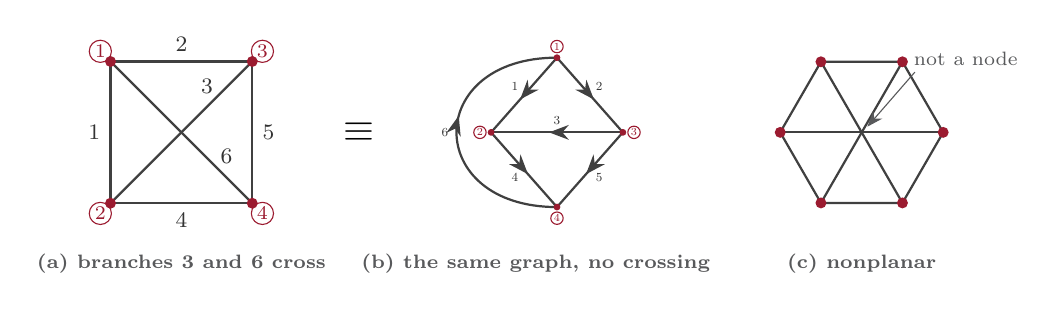
\begin{tikzpicture}[scale=0.9]
  \begin{scope}
    \squarekfour
    \node[ttl] at (1,-0.85) {(a) branches 3 and 6 cross};
  \end{scope}
  \node[font=\Large] at (3.5,1) {$\equiv$};
  \begin{scope}[xshift=6.3cm, yshift=1cm, scale=0.62, transform shape]
    \bridgecoords \bridgegraph
  \end{scope}
  \node[ttl] at (6.0,-0.85) {(b) the same graph, no crossing};
  \begin{scope}[xshift=10.6cm, yshift=1cm]
    \foreach \a in {0,60,...,300} \coordinate (h\a) at (\a:1.15);
    \draw[black!75, thick] (h0) -- (h60) -- (h120) -- (h180) -- (h240) -- (h300) -- cycle;
    \draw[black!75, thick] (h0) -- (h180); \draw[black!75, thick] (h60) -- (h240);
    \draw[black!75, thick] (h120) -- (h300);
    \foreach \a in {0,60,...,300} \fill[metured] (h\a) circle (2.2pt);
    \draw[-{Stealth[length=2mm]}, metugray] (0.75,0.85) -- (0.08,0.08);
    \node[capn, anchor=south west] at (0.6,0.8) {not a node};
    \node[ttl] at (0,-1.85) {(c) nonplanar};
  \end{scope}
\end{tikzpicture}
\end{center}

(a) is the graph of the bridge circuit, drawn as a square: its two diagonals,
branches~3 and~6, cross. (b) is the same graph --- same nodes, same branches --- with
branch~6 taken around the outside. No branches cross, so the graph is planar.

(c) has six nodes on a hexagon and three long diagonals that cross at the centre, which is
not a node. However it is redrawn, two branches always cross: the graph is
\textbf{nonplanar}.
\end{examplebox}

\subsection{Crossing is not touching}

In drawing (a), branches 3 and 6 cross only on paper. They are two separate wires, and the
crossing point is not a node. Circuit diagrams show this with a small \textbf{hop}: one wire
jumps over the other. In real hardware the hop is a jumper wire, or a track on a second
layer of the circuit board.

\begin{center}
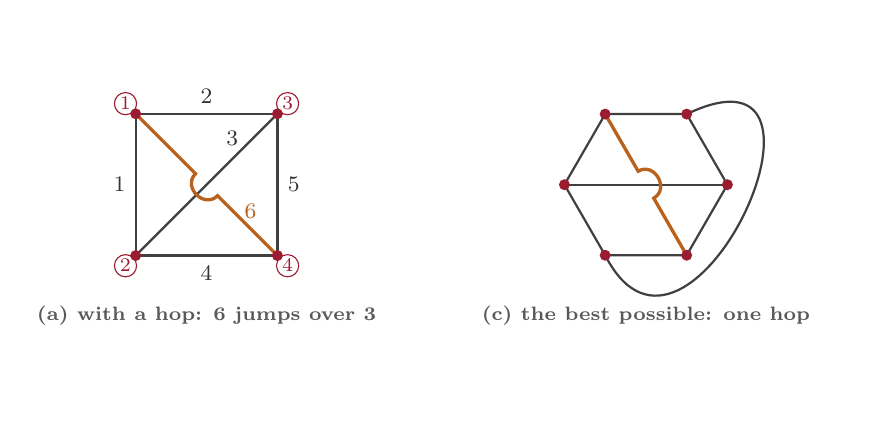
\begin{tikzpicture}[scale=0.9]
  \begin{scope}
    \squarehop
    \node[ttl] at (1,-0.85) {(a) with a hop: 6 jumps over 3};
  \end{scope}
  \begin{scope}[xshift=7.2cm, yshift=1cm]
    \hexhop
    \node[ttl] at (0,-1.85) {(c) the best possible: one hop};
  \end{scope}
\end{tikzpicture}
\end{center}

A graph is planar exactly when \emph{some} drawing needs no hop. Drawing (a) needs one, the
drawing (b) of the same graph needs none. The hexagon graph needs at least one hop however
it is drawn.

A hop is a step into the third dimension. Lift two diagonals of the hexagon graph to
different heights and no two branches meet. Seen from above, the picture is drawing (c)
again, with its crossings; from the side, the heights show.

\begin{center}
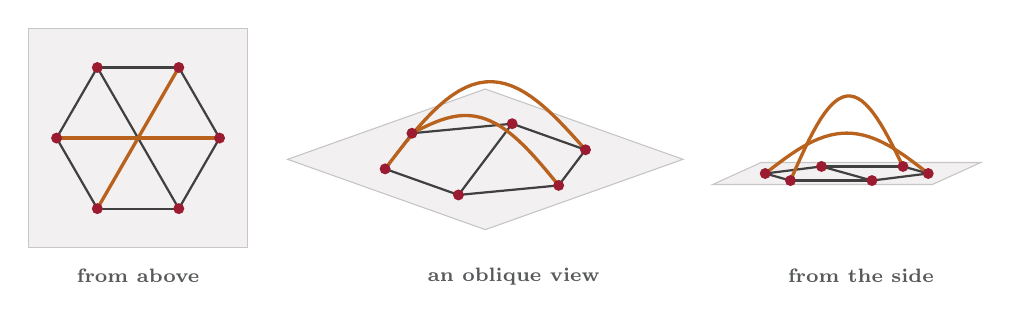
\begin{tikzpicture}[scale=0.9]
  \begin{scope}
    \hexthreeD{view top}
    \node[ttl] at (0,-1.95) {from above};
  \end{scope}
  \begin{scope}[xshift=4.9cm, yshift=-0.3cm]
    \hexthreeD{view oblique}
    \node[ttl] at (0.4,-1.65) {an oblique view};
  \end{scope}
  \begin{scope}[xshift=10.0cm, yshift=-0.5cm]
    \hexthreeD{view side}
    \node[ttl] at (0.2,-1.45) {from the side};
  \end{scope}
\end{tikzpicture}
\end{center}

%==============================================================
\section{Nonseparable graphs}\label{sec:nonsep}

\begin{definitionbox}{Nonseparable graph}
A connected graph is \textbf{nonseparable} if it stays connected after removing any one
node, together with all the branches attached to that node.
\end{definitionbox}

\begin{center}
\nsepfigure{}{}{}{}
\end{center}

Removing the centre node of the left graph removes its four branches and leaves two
separate pieces, so that graph is separable. In the bridge graph, removing \nd2 removes branches
1, 3 and 4; branches 2, 5, 6 still join \nd1, \nd3, \nd4. The same holds for any other node,
so the bridge graph is nonseparable.

From now on the graph $G$ is \textbf{planar and nonseparable}, and it is drawn without
crossings.

%==============================================================
\section{Meshes}

A planar drawing divides the plane into regions. Each region inside the graph is bounded by
a loop of branches and contains no branch inside it. That loop is an \textbf{inner mesh}
(or simply a mesh). The region outside the graph is not counted.

\begin{center}
\begin{minipage}[c]{0.4\linewidth}
\centering
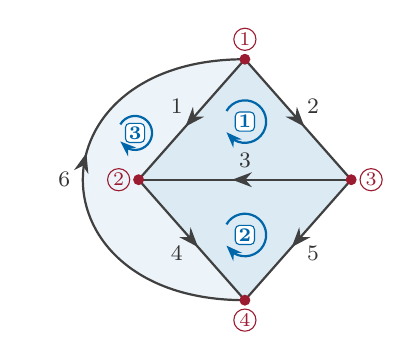
\begin{tikzpicture}[scale=0.9]
  \bridgecoords
  \fillmeshA \fillmeshB \fillmeshC[ccur!7]
  \bridgegraph \bridgemeshes
\end{tikzpicture}
\end{minipage}%
\begin{minipage}[c]{0.56\linewidth}
The bridge graph has three inner meshes:
\begin{itemize}
  \item mesh \mlab{1}: branches 1, 2, 3;
  \item mesh \mlab{2}: branches 3, 4, 5;
  \item mesh \mlab{3}: branches 1, 4, 6.
\end{itemize}
Each mesh gets a direction. By convention it is \textbf{clockwise}.
\end{minipage}
\end{center}

The number of inner meshes is
\[
  \ell = b - n + 1 \qquad (\text{here } 6 - 4 + 1 = 3),
\]
the same as the number of independent KVL equations found earlier. A mesh is a loop, so
each mesh gives one KVL equation, and these $\ell$ equations are independent.

\subsection{Why planar and nonseparable?}

\textbf{Planar.} A mesh is a region of a drawing with no crossings. A nonplanar graph cannot
be drawn without crossings, so it has no meshes. Its KVL equations are found another way,
with trees, later on.

\textbf{Nonseparable.} This is a safe, conservative assumption: sufficient, not strictly
necessary. It guarantees that every mesh is bounded by a single loop. A separable graph may
or may not satisfy this, as the two examples below show.

\begin{center}
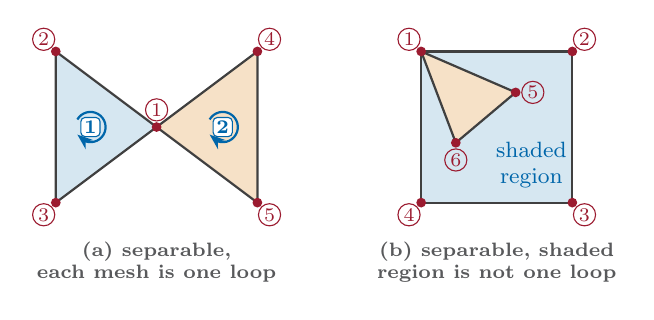
\begin{tikzpicture}[scale=0.8]
  % (a) two triangles sharing a node
  \begin{scope}
    \coordinate (p1) at (1.6,1.2); \coordinate (p2) at (0,2.4); \coordinate (p3) at (0,0);
    \coordinate (p4) at (3.2,2.4); \coordinate (p5) at (3.2,0);
    \fill[ccur!16] (p1) -- (p2) -- (p3) -- cycle;
    \fill[cvolt!22] (p1) -- (p4) -- (p5) -- cycle;
    \draw[black!75, thick] (p1) -- (p2) -- (p3) -- cycle;
    \draw[black!75, thick] (p1) -- (p4) -- (p5) -- cycle;
    \foreach \k/\pos in {1/above, 2/above left, 3/below left, 4/above right, 5/below right}
      {\fill[metured] (p\k) circle (2.2pt); \node[nlab, \pos=2pt] at (p\k) {\k};}
    \meshcw[0.24]{0.55}{1.2}{1} \meshcw[0.24]{2.65}{1.2}{2}
    \node[ttl, align=center] at (1.6,-0.95) {(a) separable,\\ each mesh is one loop};
  \end{scope}
  % (b) square with a triangle inside
  \begin{scope}[xshift=5.8cm]
    \coordinate (q1) at (0,2.4); \coordinate (q2) at (2.4,2.4);
    \coordinate (q3) at (2.4,0); \coordinate (q4) at (0,0);
    \coordinate (q5) at (1.5,1.75); \coordinate (q6) at (0.55,0.95);
    \fill[ccur!16] (q1) -- (q2) -- (q3) -- (q4) -- cycle;
    \fill[cvolt!22] (q1) -- (q5) -- (q6) -- cycle;
    \draw[black!75, thick] (q1) -- (q2) -- (q3) -- (q4) -- cycle;
    \draw[black!75, thick] (q1) -- (q5) -- (q6) -- cycle;
    \foreach \k/\pos in {1/above left, 2/above right, 3/below right, 4/below left,
                         5/right, 6/below}
      {\fill[metured] (q\k) circle (2.2pt); \node[nlab, \pos=2pt] at (q\k) {\k};}
    \node[font=\footnotesize, text=ccur, align=center] at (1.75,0.6) {shaded\\ region};
    \node[ttl, align=center] at (1.2,-0.95) {(b) separable, shaded\\ region is not one loop};
  \end{scope}
\end{tikzpicture}
\end{center}

\begin{itemize}
  \item \textbf{(a) Two triangles sharing \nd1.} Removing \nd1 splits the graph, so it is
        separable. Still, each mesh is a triangle, a single loop. The meshes work directly:
        $\ell = 2 = b - n + 1 = 6 - 5 + 1$.
  \item \textbf{(b) A triangle inside a square, attached at \nd1.} Again \nd1 is a
        \textbf{cut node}. The shaded region is bounded by the square \emph{and} the
        triangle: two loops that touch only at \nd1. It is not a single loop, so it is not a
        proper mesh.
\end{itemize}
So the nonseparable assumption rules out case (b). Graphs like (b) can still be handled ---
there is a simple fix, which we will see in a coming lecture.

%==============================================================
\section{The mesh matrix}

\begin{definitionbox}{Mesh matrix}
For a planar, nonseparable graph with $\ell$ inner meshes and $b$ branches, the
\textbf{mesh matrix} $M$ is the $\ell \times b$ matrix with entries
\[
  m_{jk} =
  \begin{cases}
    +1 & \text{if branch } k \text{ is in mesh } j \text{ and their directions coincide},\\
    -1 & \text{if branch } k \text{ is in mesh } j \text{ and their directions are opposite},\\
    \phantom{+}0 & \text{otherwise.}
  \end{cases}
\]
\end{definitionbox}

A row is a mesh: walk around it clockwise, and record each branch you meet with $+1$ if its
arrow points the way you walk, $-1$ if it points against you.

\begin{examplebox}[Example 8.2 --- the mesh matrix of the bridge]
\begin{center}
\begin{minipage}[c]{0.36\linewidth}
\centering
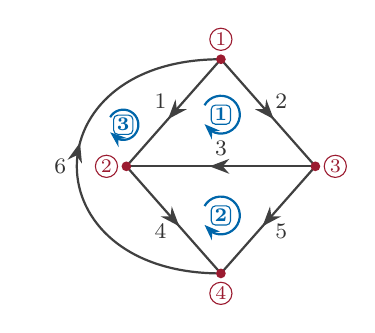
\begin{tikzpicture}[scale=0.8]
  \bridgecoords
  \bridgegraph \bridgemeshes
\end{tikzpicture}
\end{minipage}%
\begin{minipage}[c]{0.62\linewidth}
\small
\textbf{Mesh \mlab{1}} (clockwise: \nd1 $\to$ \nd3 $\to$ \nd2 $\to$ \nd1). Branches 2 and 3
point along the walk: $+1$. Branch~1 points from \nd1 to \nd2, against the walk: $-1$.\\[3pt]
\textbf{Mesh \mlab{2}} (\nd2 $\to$ \nd3 $\to$ \nd4 $\to$ \nd2). Branch~5: $+1$. Branches 3
and 4: $-1$.\\[3pt]
\textbf{Mesh \mlab{3}} (\nd4 $\to$ \nd1 $\to$ \nd2 $\to$ \nd4, along branch~6 first).
Branches 6, 1 and 4 all point along the walk: $+1$.
\end{minipage}
\end{center}
\[
  M = \incmatm{Mn}{6}{1,2,3}{%
     -1 \&  1 \&  1 \&  0 \&  0 \&  0\\
      0 \&  0 \& -1 \& -1 \&  1 \&  0\\
      1 \&  0 \&  0 \&  1 \&  0 \&  1\\}
  \qquad (3 \times 6)
\]
\end{examplebox}

\begin{ideabox}[KVL in matrix form, with meshes]
With the branch voltage vector $\Vcol{\mathbf{v}} = [\,\Vcol{v_1}\ \cdots\ \Vcol{v_b}\,]^T$,
KVL around every mesh is
\[
  \boxed{\;M\Vcol{\mathbf{v}} = \mathbf{0}\;}
\]
\end{ideabox}

For the bridge the three rows are
\[
  -\Vcol{v_1} + \Vcol{v_2} + \Vcol{v_3} = 0, \qquad
  -\Vcol{v_3} - \Vcol{v_4} + \Vcol{v_5} = 0, \qquad
  \Vcol{v_1} + \Vcol{v_4} + \Vcol{v_6} = 0 .
\]
Each is KVL around one mesh: going clockwise, a branch voltage counts with $+$ when the
walk goes from its $+$ to its $-$ (along the arrow), and with $-$ otherwise.

%==============================================================
\section{Mesh currents}

\begin{definitionbox}{Mesh current}
To each inner mesh assign a \textbf{mesh current}: a current that circulates around that
mesh in its (clockwise) direction. The mesh current vector is
$\Icol{\mathbf{i}_M} = [\,\Icol{i_{M1}}\ \cdots\ \Icol{i_{M\ell}}\,]^T$.
\end{definitionbox}

Every branch current is a sum of mesh currents. A branch carries the mesh currents of the
meshes it belongs to: $+$ if the mesh direction coincides with the branch arrow, $-$ if not.
These are exactly the entries of column $j$ of $M$.

\begin{examplebox}[Example 8.3 --- branch currents of the bridge from mesh currents]
\begin{center}
\begin{minipage}[c]{0.3\linewidth}
\centering
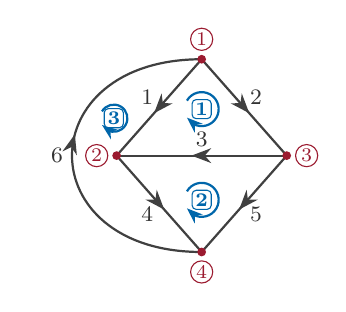
\begin{tikzpicture}[scale=0.72]
  \bridgecoords
  \bridgegraph \bridgemeshes
\end{tikzpicture}
\end{minipage}%
\begin{minipage}[c]{0.68\linewidth}
\[
  \left.
  \begin{aligned}
    \Icol{i_1} &= -\Icol{i_{M1}} + \Icol{i_{M3}}\\
    \Icol{i_2} &= \Icol{i_{M1}}\\
    \Icol{i_3} &= \Icol{i_{M1}} - \Icol{i_{M2}}\\
    \Icol{i_4} &= -\Icol{i_{M2}} + \Icol{i_{M3}}\\
    \Icol{i_5} &= \Icol{i_{M2}}\\
    \Icol{i_6} &= \Icol{i_{M3}}
  \end{aligned}
  \ \right\}
  \;\Longrightarrow\;
  \begin{bmatrix}
    \Icol{i_1}\\ \Icol{i_2}\\ \Icol{i_3}\\ \Icol{i_4}\\ \Icol{i_5}\\ \Icol{i_6}
  \end{bmatrix}
  =
  \underbrace{\begin{bmatrix}
    -1 &  0 & 1\\
     1 &  0 & 0\\
     1 & -1 & 0\\
     0 & -1 & 1\\
     0 &  1 & 0\\
     0 &  0 & 1
  \end{bmatrix}}_{M^T}
  \begin{bmatrix} \Icol{i_{M1}}\\ \Icol{i_{M2}}\\ \Icol{i_{M3}} \end{bmatrix}
\]
\end{minipage}
\end{center}
Branch~3 is shared by meshes \mlab{1} and \mlab{2}. Mesh \mlab{1} goes along its arrow and
mesh \mlab{2} against it, so $\Icol{i_3} = \Icol{i_{M1}} - \Icol{i_{M2}}$. Branch~2 is only in
mesh \mlab{1}, so $\Icol{i_2} = \Icol{i_{M1}}$.
\end{examplebox}

\begin{ideabox}[Branch currents from mesh currents]
\[
  \boxed{\;\Icol{\mathbf{i}} = M^T\,\Icol{\mathbf{i}_M}\;}
  \qquad
  \Icol{\mathbf{i}} \in \mathbb{R}^{b}:\ \text{branch current vector},
  \qquad
  \Icol{\mathbf{i}_M} \in \mathbb{R}^{\ell}:\ \text{mesh current vector}.
\]
\end{ideabox}

\textbf{Remarks.}
\begin{itemize}
  \item Once the $\ell$ mesh currents are known, all $b$ branch currents are known.
  \item KCL puts \textbf{no constraint} on the mesh currents. A mesh current enters each
        node on its loop and leaves it again, so it adds zero to KCL at every node. For
        example, KCL at \nd2 of the bridge:
        $-\Icol{i_1} - \Icol{i_3} + \Icol{i_4}
        = (\Icol{i_{M1}} - \Icol{i_{M3}}) - (\Icol{i_{M1}} - \Icol{i_{M2}})
          + (-\Icol{i_{M2}} + \Icol{i_{M3}}) = 0$.
  \item In matrix form: $\mathbf{0} = A\Icol{\mathbf{i}} = AM^T\Icol{\mathbf{i}_M}$ for every
        $\Icol{\mathbf{i}_M}$. A matrix that gives zero for every vector is the zero matrix,
        so $AM^T = \mathbf{0}$. Write the rows of $A$ and $M$ as vectors,
        \[
          A = \begin{bmatrix} \mathbf{a}_1^T\\ \mathbf{a}_2^T\\ \mathbf{a}_3^T \end{bmatrix},
          \qquad
          M = \begin{bmatrix} \mathbf{m}_1^T\\ \mathbf{m}_2^T\\ \mathbf{m}_3^T \end{bmatrix},
          \qquad
          (AM^T)_{jr} = \mathbf{a}_j^T\mathbf{m}_r = 0 \quad \text{for all } j, r .
        \]
        Every row of $A$ is \textbf{orthogonal} to every row of $M$. For example,
        \[
          \mathbf{a}_2^T\mathbf{m}_1
          = \begin{bmatrix} -1 & 0 & -1 & 1 & 0 & 0 \end{bmatrix}
            \begin{bmatrix} -1 & 1 & 1 & 0 & 0 & 0 \end{bmatrix}^T
          = (-1)(-1) + (-1)(1) = 0 .
        \]
        A node and a mesh share either no branch or two, and the two terms cancel.
\end{itemize}
So the mesh currents are a good choice of unknowns: there are only $\ell = b - n + 1$ of them,
they are free, and KCL is then satisfied automatically. This is the idea behind mesh
analysis.

\begin{examplebox}[Example 8.4 --- mesh currents in a familiar circuit]
The circuit below was solved earlier with node voltages:
$\Icol{i_1} = \Icol{i_2} = 2\A$, $\Icol{i_3} = 1.5\A$, $\Icol{i_4} = 0.5\A$, and
$\Vcol{\mathbf{v}} = [\,{-10}\ \ 4\ \ 6\ \ 6\,]^T\V$. Write $M$, express the branch currents
with mesh currents, and check both results.

\begin{center}
\tcircuit{0.9}
\end{center}

Mesh \mlab{1} (left, clockwise) goes up through the source, right through $2\ohm$ and down
through $4\ohm$: branches 1, 2, 3 all along their arrows. Mesh \mlab{2} goes up through the
$4\ohm$ (against branch~3) and down through the $12\ohm$ (along branch~4):
\[
  M =
  \begin{bmatrix}
    1 & 1 &  1 & 0\\
    0 & 0 & -1 & 1
  \end{bmatrix},
  \qquad
  \Icol{\mathbf{i}} = M^T\Icol{\mathbf{i}_M}:\quad
  \Icol{i_1} = \Icol{i_2} = \Icol{i_{M1}},\ \
  \Icol{i_3} = \Icol{i_{M1}} - \Icol{i_{M2}},\ \
  \Icol{i_4} = \Icol{i_{M2}} .
\]
With $\Icol{i_{M1}} = 2\A$ and $\Icol{i_{M2}} = 0.5\A$ this gives exactly the branch currents
above. KVL: $M\Vcol{\mathbf{v}} = [\,{-10} + 4 + 6,\ \ {-6} + 6\,]^T = \mathbf{0}$.
\end{examplebox}

%==============================================================
\section{Looking ahead: why mesh currents?}

The same idea as with node voltages, with the roles of KCL and KVL swapped. Again there are
$2b$ unknowns and $2b$ equations: $b$ element, $n-1$ KCL and $\ell = b-n+1$ KVL.

\begin{center}

\begin{tikzpicture}[scale=0.92, transform shape,
    fb/.style={draw=metugray, fill=metulight, rounded corners=3pt, align=center,
               minimum height=1.15cm, text width=1.95cm, font=\small},
    fa/.style={-{Stealth[length=2.5mm]}, very thick, metugray},
    fl/.style={font=\footnotesize, align=center, text=metured}]
  \node[fb, draw=metured, very thick] (u) at (0,0) {$\Icol{\mathbf{i}_M}$\\ $\ell$ unknowns};
  \node[fb] (a) at (4.6,0) {all $b$ branch\\ currents $\Icol{\mathbf{i}}$};
  \node[fb] (b) at (9.2,0) {all $b$ branch\\ voltages $\Vcol{\mathbf{v}}$};
  \node[fb, draw=metured, very thick] (c) at (13.8,0) {$\ell$ equations\\ for $\Icol{\mathbf{i}_M}$};
  \draw[fa] (u) -- node[fl, above=2pt] {KCL holds\\ for any $\Icol{\mathbf{i}_M}$:\\ $\Icol{\mathbf{i}} = M^T\Icol{\mathbf{i}_M}$} (a);
  \draw[fa] (a) -- node[fl, above=2pt] {element\\ equations} (b);
  \draw[fa] (b) -- node[fl, above=2pt] {KVL:\\ $M\Vcol{\mathbf{v}} = \mathbf{0}$} (c);
\end{tikzpicture}
\end{center}

\begin{itemize}
  \item \textbf{KCL.} Take the $\ell$ mesh currents as the unknowns and write every branch
        current as $\Icol{\mathbf{i}} = M^T\Icol{\mathbf{i}_M}$. This satisfies KCL at every
        node for \emph{any} $\Icol{\mathbf{i}_M}$. So no KCL equation has to be written: the
        $n-1$ KCL equations hold automatically.
  \item \textbf{Element equations.} These are still used: they give each branch voltage from
        its current, hence in terms of $\Icol{\mathbf{i}_M}$. For a resistor shared by meshes
        1 and 2, e.g.\ $\Vcol{v_k} = R_k\Icol{i_k} = R_k(\Icol{i_{M1}} - \Icol{i_{M2}})$.
  \item \textbf{KVL.} Put these voltages into $M\Vcol{\mathbf{v}} = \mathbf{0}$. This leaves
        $\ell$ equations, exactly as many as the unknowns $\Icol{\mathbf{i}_M}$.
\end{itemize}
Solve them for $\Icol{\mathbf{i}_M}$, and every other current and voltage follows. So $2b$
unknowns become $\ell = b - n + 1$, and $\ell < b$ because a circuit has $n \ge 2$ nodes.
Node voltages need $n - 1$ unknowns, mesh currents $\ell$: which choice is shorter depends
on the circuit. In Example~8.4, $\ell = 2$ and $n - 1 = 2$, but the source fixes one node
voltage, so a single node voltage is enough there. This is \textbf{mesh analysis}, the subject of a coming
lecture.

%==============================================================
\section*{Summary}
\addcontentsline{toc}{section}{Summary}

\begin{center}
\small
\renewcommand{\arraystretch}{1.25}
\begin{tabular}{@{}l l l@{}}
\toprule
 & \textbf{node voltages} & \textbf{mesh currents}\\
\midrule
works for                & any connected graph       & planar, nonseparable graphs\\
how many unknowns        & $n - 1$                   & $\ell = b - n + 1$\\
matrix                   & $A$ \ ($(n-1)\times b$)   & $M$ \ ($\ell\times b$)\\
satisfied automatically  & KVL: $\Vcol{\mathbf{v}} = A^T\Vcol{\mathbf{e}}$
                         & KCL: $\Icol{\mathbf{i}} = M^T\Icol{\mathbf{i}_M}$\\
left to write            & KCL: $A\Icol{\mathbf{i}} = \mathbf{0}$
                         & KVL: $M\Vcol{\mathbf{v}} = \mathbf{0}$\\
\bottomrule
\end{tabular}
\end{center}

\begin{itemize}
  \item A graph is \textbf{planar} if it can be drawn with no crossings, and
        \textbf{nonseparable} if removing any one node leaves it connected.
  \item The inner meshes of a planar drawing, taken clockwise, give the \textbf{mesh matrix}
        $M$: $+1$ along, $-1$ against, $0$ otherwise. KVL is $M\Vcol{\mathbf{v}} = \mathbf{0}$.
  \item \textbf{Mesh currents} circulate around the meshes; $\Icol{\mathbf{i}} =
        M^T\Icol{\mathbf{i}_M}$. KCL puts no constraint on them, so $AM^T = \mathbf{0}$.
  \item \textbf{Why}: with the $\ell$ mesh currents as unknowns, KCL holds automatically (no KCL equation
        to write), and KVL gives
        just enough equations --- the idea of mesh analysis.
\end{itemize}

\subsection*{Next lecture}
Nonplanar circuits: \textbf{trees}, \textbf{cutsets} and fundamental cutsets --- tools that
work for any connected graph.

%==============================================================
\section*{Appendix: why the rows of $A$ and $M$ are orthogonal}
\addcontentsline{toc}{section}{Appendix: why the rows of $A$ and $M$ are orthogonal}

The product $\mathbf{a}_j^T\mathbf{m}_r$ adds $a_{jk}\,m_{rk}$ over the branches $k$. Here $a_{jk} = +1$ if branch $k$ leaves node $j$. A term
is nonzero only if branch $k$ touches node $j$ \emph{and} lies on mesh $r$. If mesh $r$ misses
node $j$, all terms are zero. Otherwise the walk around mesh $r$ comes into node $j$ on one
branch and goes out on another; a mesh passes a node only once, so these are the only two terms.
\par\smallskip\noindent
\begin{minipage}[c]{0.4\linewidth}
\centering
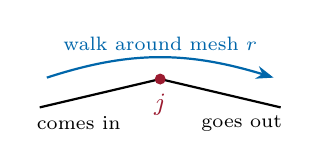
\begin{tikzpicture}[scale=0.9]
  \coordinate (J) at (0,0);
  \draw[thick] (-1.7,-0.4) -- (J) -- (1.7,-0.4);
  \fill[metured] (J) circle (2.2pt);
  \node[font=\small, text=metured, below=2pt] at (J) {$j$};
  \draw[ccur, thick, -{Stealth[length=2.2mm]}] (-1.6,0.02) to[out=18, in=162] (1.6,0.02);
  \node[font=\scriptsize, text=ccur] at (0,0.5) {walk around mesh $r$};
  \node[font=\scriptsize] at (-1.15,-0.62) {comes in};
  \node[font=\scriptsize] at (1.15,-0.62) {goes out};
\end{tikzpicture}
\end{minipage}%
\hfill
\begin{minipage}[c]{0.57\linewidth}
\centering\small
\renewcommand{\arraystretch}{1.3}\setlength{\tabcolsep}{5pt}
\begin{tabular}{@{}l c c@{}}
\toprule
$a_{jk}\,m_{rk}$ & arrow along walk & arrow against walk\\
\midrule
walk goes out of $j$ & $(+1)(+1) = +1$ & $(-1)(-1) = +1$\\
walk comes into $j$  & $(-1)(+1) = -1$ & $(+1)(-1) = -1$\\
\bottomrule
\end{tabular}
\end{minipage}\par\smallskip
\noindent Whatever the arrows, the branch the walk goes out on gives $+1$ and the one it comes in on
gives $-1$, so $\mathbf{a}_j^T\mathbf{m}_r = 0$. The same holds for any loop, not only meshes.

\end{document}
